En este capítulo se presentan las bases tecnológicas sobre las que se sustenta
Voctomix~2.0. Se analizan los tres eslabones de la cadena de producción audiovisual
en directo: el modelo de producción y las herramientas de realización disponibles
(Sección~\ref{sec:produccion_av}), los estándares e interfaces de contribución de señal
(Sección~\ref{sec:contribucion_av}), y los protocolos y códecs empleados en la
distribución del contenido al espectador final (Sección~\ref{sec:distribucion_av}). El
objetivo es que el lector comprenda el contexto técnico en el que se enmarca el
trabajo antes de abordar el diseño e implementación del sistema en el
Capítulo~\ref{chap:diseno}.

\section{Producción audiovisual}
\label{sec:produccion_av}

La producción audiovisual en directo engloba el conjunto de procesos técnicos y
organizativos que permiten capturar, procesar y distribuir contenido de vídeo y audio
en tiempo real. Históricamente anclada a infraestructuras físicas costosas y al
desplazamiento de equipos al lugar del evento, esta disciplina ha experimentado en la
última década una transformación radical impulsada por la convergencia entre las redes
de datos y los flujos de media profesionales~\cite{tmbroadcast_remi}.

\subsection{Producción audiovisual tradicional}

El modelo de producción tradicional se basa en el despliegue físico de toda la
infraestructura técnica y del personal en el emplazamiento del evento. El componente
central de este modelo es el \textbf{mezclador hardware}, denominado
\textit{switcher} (conmutador de vídeo), un dispositivo dedicado que selecciona en cada instante qué fuente
de vídeo se emite a la salida de programa y gestiona las transiciones y los efectos.
Fabricantes como Blackmagic Design (ATEM), Ross Video o Grass Valley (Kayenne) dominan
el mercado de estos equipos, que ofrecen latencias sub-imagen, múltiples buses de
programa y previsualización simultáneos, y redundancia hardware certificada para
operación continua~\cite{blackmagic_atem}.

En el modelo tradicional, todas las fuentes, cámaras, reproductores de vídeo y
ordenadores de presentación, se interconectan mediante cableado \textbf{SDI}
(\textit{Serial Digital Interface}), el estándar histórico de la industria \textit{broadcast} (radiodifusión)
para el transporte de vídeo sin comprimir~\cite{smpte_sdi}. La señal resultante recorre
el mezclador, los sistemas de rotulación y grabación, y finalmente el encoder de
distribución, todo ello dentro del mismo emplazamiento físico.

Este modelo ha demostrado su solidez durante décadas en las grandes producciones de
televisión: retransmisiones deportivas, eventos parlamentarios y galas de premios
emplean esta arquitectura con decenas de fuentes de cámara gestionadas en tiempo real.
Sin embargo, su principal limitación es económica y logística: el coste de adquirir y
transportar el equipamiento, más el personal técnico necesario para su instalación y
operación, lo pone fuera del alcance de organizaciones de mediana escala.

Un caso ilustrativo es la retransmisión de un partido de La Liga de fútbol profesional
en España. Este tipo de producción moviliza habitualmente entre 20 y 30 cámaras SDI,
varias unidades móviles de producción equipadas con mezcladores hardware de gama alta
y un equipo técnico de entre 50 y 100 personas desplazadas al estadio~\cite{blackmagic_atem}.
El coste de una unidad móvil de estas características puede superar los 2 millones de
euros, cifra a la que se suma el gasto recurrente en desplazamientos, montaje y
operación. Este modelo queda así reservado a grandes cadenas de televisión y
organizaciones con infraestructura broadcast consolidada, resultando inaccesible para
entidades académicas, asociaciones o eventos de mediana escala.

\subsection{Producción audiovisual remota}

La producción remota, conocida en la industria por el acrónimo
\textbf{REMI} (\textit{Remote Integration Model}), surge para resolver estas
limitaciones permitiendo que la realización se lleve a cabo desde un centro de
producción centralizado, mientras en el lugar del evento solo se mantiene el equipo
técnico mínimo necesario para la captura de
señal~\cite{tmbroadcast_remi,remi_workflow_ibc2023}.

\subsubsection*{Arquitectura técnica del modelo REMI}

La figura~\ref{fig:remi_arquitectura} ilustra la separación funcional entre el lugar
del evento y el centro de producción remoto. En el emplazamiento solo permanecen las
cámaras, los micrófonos y un sistema de contribución IP que codifica y transmite la
señal hacia el centro remoto. El procesamiento completo, mezcla de fuentes, inserción
de gráficos, control de audio, gestión de overlays y distribución al espectador,
se realiza de forma centralizada.

\begin{figure}[H]
  \centering
  \hspace*{-1.5cm}
  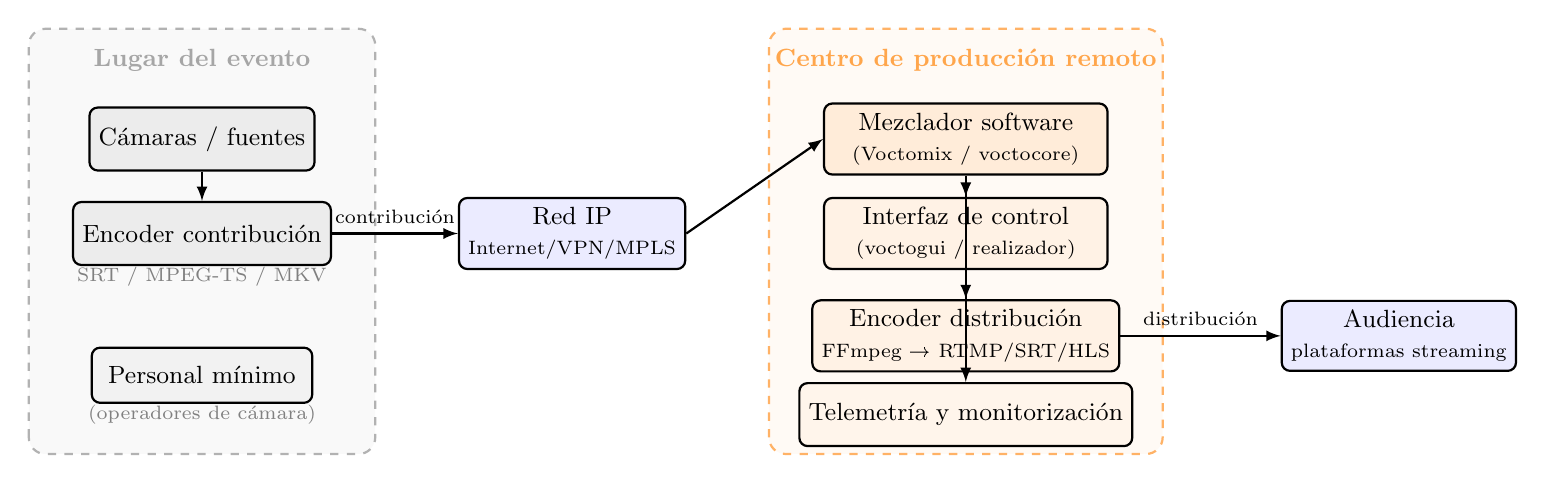
\begin{tikzpicture}[>=latex, thick, font=\small]
    % ── Lugar del evento (izquierda) ─────────────────────────────────
    \draw[rounded corners=6pt, dashed, gray!60, fill=gray!5]
      (-0.4,-2.0) rectangle (4.0,3.4);
    \node[font=\small\bfseries, gray!70] at (1.8,3.0) {Lugar del evento};

    \node[draw, rounded corners=3pt, minimum width=2.8cm, minimum height=0.8cm,
          align=center, fill=gray!15] (cam1) at (1.8, 2.0) {Cámaras / fuentes};
    \node[draw, rounded corners=3pt, minimum width=2.8cm, minimum height=0.8cm,
          align=center, fill=gray!15] (enc)  at (1.8, 0.8) {Encoder contribución};
    \node[font=\scriptsize, text=gray] at (1.8, 0.25) {SRT / MPEG-TS / MKV};
    \node[draw, rounded corners=3pt, minimum width=2.8cm, minimum height=0.7cm,
          align=center, fill=gray!10] (crew) at (1.8,-1.0) {Personal mínimo};
    \node[font=\scriptsize, text=gray] at (1.8,-1.5) {(operadores de cámara)};

    \draw[->] (cam1.south) -- (enc.north);

    % ── Red IP (centro) ───────────────────────────────────────────────
    \node[draw, rounded corners=3pt, minimum width=1.8cm, minimum height=0.8cm,
          align=center, fill=blue!8] (net) at (6.5, 0.8) {Red IP\\{\scriptsize Internet/VPN/MPLS}};
    \draw[->] (enc.east) -- (net.west)
      node[midway, above, font=\scriptsize] {contribución};

    % ── Centro de producción (derecha) ───────────────────────────────
    \draw[rounded corners=6pt, dashed, orange!60, fill=orange!4]
      (9.0,-2.0) rectangle (14.0,3.4);
    \node[font=\small\bfseries, orange!70] at (11.5,3.0) {Centro de producción remoto};

    \node[draw, rounded corners=3pt, minimum width=3.6cm, minimum height=0.8cm,
          align=center, fill=orange!15] (mix) at (11.5, 2.0)
          {Mezclador software\\{\scriptsize (Voctomix / voctocore)}};
    \node[draw, rounded corners=3pt, minimum width=3.6cm, minimum height=0.8cm,
          align=center, fill=orange!10] (gui) at (11.5, 0.8)
          {Interfaz de control\\{\scriptsize (voctogui / realizador)}};
    \node[draw, rounded corners=3pt, minimum width=3.6cm, minimum height=0.8cm,
          align=center, fill=orange!10] (dist) at (11.5,-0.5)
          {Encoder distribución\\{\scriptsize FFmpeg → RTMP/SRT/HLS}};
    \node[draw, rounded corners=3pt, minimum width=3.6cm, minimum height=0.8cm,
          align=center, fill=orange!8] (tel) at (11.5,-1.5)
          {Telemetría y monitorización};

    \draw[->] (net.east) -- (mix.west);
    \draw[->] (mix.south) -- (gui.north);
    \draw[->] (mix.south) -- ++(0,-0.3) -| (dist.north);
    \draw[->] (gui.south)  -- ++(0,-0.15) -| (tel.north);

    % ── Audiencia (derecha del centro de producción) ─────────────────
    \node[draw, rounded corners=3pt, minimum width=2.2cm, minimum height=0.8cm,
          align=center, fill=blue!8] (aud) at (17.0, -0.5)
          {Audiencia\\{\scriptsize plataformas streaming}};
    \draw[->] (dist.east) -- (aud.west)
      node[midway, above, font=\scriptsize] {distribución};
  \end{tikzpicture}
  \caption{Arquitectura del modelo REMI.}
  \label{fig:remi_arquitectura}
\end{figure}

Esta separación permite que el realizador opere el sistema desde cualquier ubicación
con acceso a la red, y que el centro de producción pueda atender simultáneamente
eventos en distintas localizaciones reutilizando la misma infraestructura de
mezclado~\cite{remi_workflow_ibc2023}.

\subsubsection*{Casos de uso reales}

La adopción del modelo REMI ha crecido exponencialmente en los últimos años. Un ejemplo
emblemático fue la producción audiovisual de los Juegos Olímpicos de Tokio 2021 por
parte de Olympic Broadcasting Services (OBS), que produjo más de 9.500 horas de
contenido con la realización, mezcla de señales y control de calidad realizados desde
el International Broadcast Centre y desde centros remotos distribuidos por todo el
mundo~\cite{obs_tokyo_2021}. En España, Telefónica Servicios Audiovisuales (TSA)
ejecutó en 2022 la producción remota multicámara de un partido de la UEFA Champions
League disputado en el estadio Santiago Bernabéu, realizando toda la dirección desde
las instalaciones de Telefónica en Tres Cantos, a más de 30~km del estadio~\cite{tsa_remi_2022}.

\subsubsection*{Ventajas del modelo remoto}

Las ventajas del modelo REMI frente a la producción tradicional son
significativas~\cite{tmbroadcast_remi,remi_workflow_ibc2023}:

\begin{itemize}
  \item \textbf{Reducción de costes:} se minimiza el desplazamiento de personal y
  equipos. Solo se requiere in situ el equipo de captura; la realización, mezcla y
  edición se realizan de forma centralizada.
  \item \textbf{Sostenibilidad:} la reducción de desplazamientos contribuye a disminuir
  la huella de carbono de las producciones, un factor cada vez más valorado por
  organizaciones y broadcasters.
  \item \textbf{Escalabilidad:} el sistema puede adaptarse a producciones de diferente
  escala reutilizando la misma infraestructura centralizada.
  \item \textbf{Flexibilidad geográfica:} es posible retransmitir eventos desde
  cualquier parte del mundo con conectividad IP, sin necesidad de desplazar el equipo
  de producción.
\end{itemize}

La adopción del modelo REMI no está exenta de retos. La Tabla~\ref{tab:remi_beneficios_desafios}
resume los principales beneficios y desafíos identificados en entornos de producción
reales~\cite{tmbroadcast_remi,remi_workflow_ibc2023}.

\begin{table}[H]
  \centering
  \caption{Beneficios y desafíos de la producción audiovisual remota (REMI).}
  \label{tab:remi_beneficios_desafios}
  \small
  \begin{tabular}{|p{2.4cm}|p{5.5cm}|p{5.5cm}|}
    \hline
    \textbf{Dimensión} & \textbf{Beneficio} & \textbf{Desafío / Dificultad} \\
    \hline
    Coste           & Reducción de desplazamientos y equipos    & Inversión inicial en red y software \\
    Latencia        & Viable con SRT ($<$1~s en WAN)            & Coordinación realizador--cámaras difícil \\
    Escalabilidad   & Un centro atiende múltiples eventos       & Riesgo de sobrecarga del servidor \\
    Red             & Producción desde cualquier ubicación IP   & Corte de red detiene la producción \\
    Calidad         & Hardware ilimitado en el centro remoto    & Artefactos con ancho de banda insuficiente \\
    Sincronía A/V   & MKV + SRT garantizan sincronía            & \textit{jitter} (fluctuación) puede desincronizar fuentes \\
    Seguridad       & Cifrado AES-256 extremo a extremo         & Mayor superficie de ataque expuesta \\
    Complejidad     & Herramientas maduras (Voctomix, FFmpeg)   & Diagnóstico de pipelines distribuidos \\
    Sostenibilidad  & Menor huella de carbono                   & Consumo energético del centro permanente \\
    \hline
  \end{tabular}
\end{table}

\subsubsection*{Herramientas de producción remota por software}

La disponibilidad de herramientas de mezclado por software ha democratizado el acceso
al modelo remoto incluso para organizaciones sin presupuesto broadcast:

\begin{itemize}
  \item \textbf{OBS Studio}~\cite{obs_studio}: solución de código abierto ampliamente
  utilizada para \textit{streaming} y grabación. Su diseño todo en uno concentra
  captura, composición y emisión en una única aplicación para un único operador.
  Soporta fuentes de entrada variadas, como cámaras USB, captura de pantalla o fuentes
  IP, con soporte para transiciones y filtros. Es la opción más utilizada por
  \textit{streamers} independientes, aunque su diseño centralizado limita su uso en
  entornos distribuidos.

  \item \textbf{vMix}~\cite{vmix_software}: solución comercial profesional para Windows
  con soporte NDI, \textit{multiview} (vista múltiple) y producción 4K. Permite gestionar múltiples
  fuentes, aplicar \textit{chroma key} (croma) y transiciones, y emitir a varias plataformas
  simultáneamente. Su coste de licencia, que puede superar los 1.000~\euro, y su
  restricción a Windows la excluyen de entornos \textit{open-source} sobre Linux.

  \item \textbf{Voctomix}~\cite{voctomix_github}: herramienta de código abierto con
  arquitectura cliente-servidor que separa el motor de mezcla (\texttt{voctocore}) de
  la interfaz de control (\texttt{voctogui}), permitiendo que el procesamiento se
  realice en un servidor mientras el operador trabaja desde otro equipo conectado por
  red. Construido sobre el \textit{framework} (entorno de software) GStreamer, proporciona composición de
  vídeo con múltiples fuentes, transiciones animadas, overlays y un protocolo de
  control TCP extensible. Es la herramienta extendida en el presente trabajo (véase el
  Capítulo~\ref{chap:diseno}). Su motor interno es \textbf{GStreamer}~\cite{gstreamer_docs},
  un \textit{framework} multimedia de código abierto que permite combinar múltiples
  fuentes de vídeo y producir una única salida de programa en tiempo real.
\end{itemize}

\begin{table}[H]
  \centering
  \caption{Comparativa entre producción audiovisual tradicional y producción remota (REMI).}
  \label{tab:trad_vs_remi}
  \begin{tabular}{|l|c|c|}
    \hline
    \textbf{Parámetro} & \textbf{Tradicional} & \textbf{REMI / Software} \\
    \hline
    Infraestructura en lugar del evento & Completa          & Mínima (cámaras + encoder) \\
    Coste de equipamiento               & Muy alto          & Bajo (hardware convencional) \\
    Personal in situ                    & Numeroso          & Reducido \\
    Latencia extremo a extremo          & Sub-imagen        & 1 fotograma -- varios segundos \\
    Escalabilidad                       & Limitada          & Alta \\
    Sostenibilidad (huella de carbono)  & Baja              & Alta \\
    Ejemplo                             & Blackmagic ATEM   & OBS, vMix, Voctomix \\
    \hline
  \end{tabular}
\end{table}

\begin{figure}[H]
  \centering
  \hspace*{-1cm}
  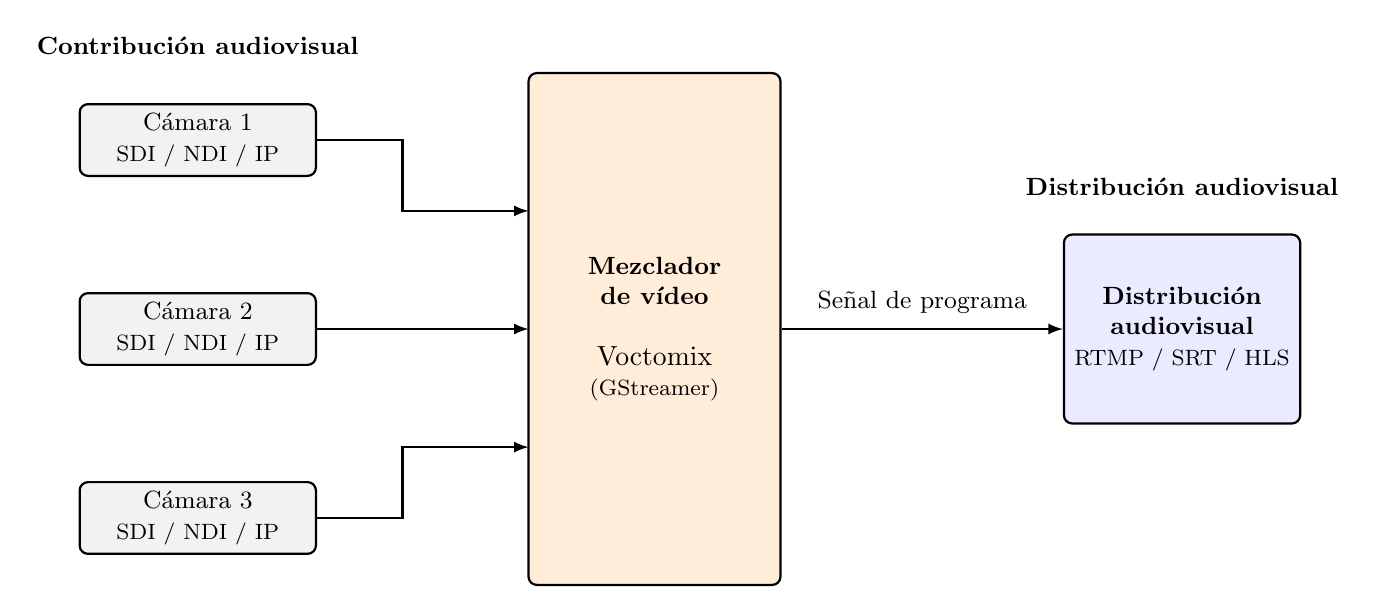
\begin{tikzpicture}[>=latex, thick, font=\small]
    \node[draw, rounded corners=3pt, minimum width=3cm, minimum height=0.9cm,
          align=center, fill=gray!10] (c1) at (0, 2.4) {Cámara 1 \\ {\footnotesize SDI / NDI / IP}};
    \node[draw, rounded corners=3pt, minimum width=3cm, minimum height=0.9cm,
          align=center, fill=gray!10] (c2) at (0, 0)   {Cámara 2 \\ {\footnotesize SDI / NDI / IP}};
    \node[draw, rounded corners=3pt, minimum width=3cm, minimum height=0.9cm,
          align=center, fill=gray!10] (c3) at (0,-2.4) {Cámara 3 \\ {\footnotesize SDI / NDI / IP}};

    \node[draw, rounded corners=3pt, minimum width=3.2cm, minimum height=6.5cm,
          align=center, fill=orange!15] (mix) at (5.8, 0)
          {\textbf{Mezclador} \\ \textbf{de vídeo} \\ \\ {\normalsize Voctomix} \\
           {\footnotesize (GStreamer)}};

    \node[draw, rounded corners=3pt, minimum width=3cm, minimum height=2.4cm,
          align=center, fill=blue!8] (dst) at (12.5, 0)
          {\textbf{Distribución} \\ \textbf{audiovisual} \\ {\footnotesize RTMP / SRT / HLS}};

    \draw[->] (c1.east) -- (2.6, 2.4) -- (2.6, 1.5) -- (4.2, 1.5);
    \draw[->] (c2.east) -- (4.2, 0);
    \draw[->] (c3.east) -- (2.6,-2.4) -- (2.6,-1.5) -- (4.2,-1.5);
    \draw[->] (mix.east) -- node[above, yshift=2pt] {Señal de programa} (dst.west);

    \node[font=\small\bfseries] at (0, 3.6)   {Contribución audiovisual};
    \node[font=\small\bfseries] at (12.5, 1.8) {Distribución audiovisual};
  \end{tikzpicture}
  \caption{Cadena de producción audiovisual en directo: señales de contribución,
           mezclador de vídeo y salida de distribución.}
  \label{fig:cadena_produccion}
\end{figure}
